\documentclass[10pt,]{report}
\usepackage[utf8]{inputenc}
\usepackage{pxfonts} 
\usepackage{graphicx} 
\usepackage[none]{hyphenat} 
\usepackage{ragged2e} 
\usepackage{titlesec} 
\usepackage{indentfirst}
\usepackage{changepage}
\usepackage{enumitem}
\usepackage{longtable}
\usepackage{caption}
\usepackage{xcolor}
\usepackage{array}
\usepackage{tabularx}
\usepackage[export]{adjustbox} 
\usepackage{multirow}
\usepackage{float}
\usepackage{xcolor,colortbl}
\usepackage{hyperref}
\usepackage{titletoc}
\usepackage{tocloft}
\usepackage[chapter,newfloat]{minted}
\setminted{
  breaklines=true,
  breakanywhere=true,
  breaksymbolleft=,
  escapeinside=||,
  autogobble=true
}
\usepackage[backend=biber,style=apa]{biblatex}
\usepackage[nottoc,numbib]{tocbibind}
\tolerance=10000
\renewcommand\arraystretch{1.3}
\sloppy \graphicspath{{images/}}
\addbibresource{bibliography/reference.bib}
\usepackage[a5paper, left=2.3cm, right=2cm, top=2.3cm, bottom=2cm, bindingoffset=20pt]{geometry}
\titleformat{\chapter}[display]{\centering\normalfont\fontsize{12}{12}\selectfont\bfseries}{\thechapter}{12pt}{\fontsize{12}{12}\selectfont}
\titlespacing*{\chapter}{0pt}{0pt}{10pt}
\renewcommand\thesection{\Alph{section}}
\renewcommand\thesubsection{\arabic{subsection}}
\renewcommand\thesubsubsection{\alph{subsubsection}}
\newenvironment{code}{\captionsetup{type=listing}}{\vspace{3mm}}
\SetupFloatingEnvironment{listing}{name=Source Code}
\setcounter{secnumdepth}{3}
\renewcommand{\contentsname}{DAFTAR ISI}
\renewcommand{\listtablename}{DAFTAR TABEL}
\renewcommand{\listfigurename}{DAFTAR GAMBAR}
\renewcommand{\thechapter}{\Roman{chapter}}
\renewcommand{\thefigure}{\arabic{chapter}.\arabic{figure}}
\renewcommand{\thetable}{\arabic{chapter}.\arabic{table}}
\renewcommand{\thelisting}{\arabic{chapter}.\arabic{listing}}
\renewcommand{\cftloftitlefont}{\hfill\Large\bfseries} % Center align and increase size of "List of Figures" title
\renewcommand{\cftlottitlefont}{\hfill\Large\bfseries} % Center align and increase size of "Tables Overview" title
\renewcommand{\cftafterloftitle}{\hfill} % Center align "List of Figures" title
\renewcommand{\cftafterlottitle}{\hfill} % Center align "Tables Overview" title
\titleformat{\section}[block]{\normalfont\bfseries\fontsize{12}{12}}{\makebox[1em][l]{\thesection.}}{10pt}{\fontsize{10}{10}\selectfont}
\titleformat{\subsection}[block]{\normalfont\fontsize{12}{12}}{\makebox[1em][l]{\thesubsection.}}{10pt}{\fontsize{10}{10}\selectfont}
\titleformat{\subsubsection}[block]{\normalfont\fontsize{12}{12}}{\makebox[1em][l]{\thesubsection.\thesubsubsection.}}{10pt}{\fontsize{10}{10}\selectfont}
\titleformat{\chapter}[block]
{\normalfont\bfseries\filcenter}
{BAB \Roman{chapter} \break}
{0em}
{}

\newcommand{\chapterNoBab}[1]{
  \par\refstepcounter{chapter}% Menambahkan counter section tapi tidak menampilkannya
  \section*{#1}% Membuat section tanpa nomor
  \addcontentsline{toc}{chapter}{\protect\numberline{\thesection}#1}% Opsi untuk menambahkan ke ToC
}
\titlespacing*{\section}{0pt}{0pt}{10pt}
\DeclareCaptionFormat{custom}
{
  \textit{#1#2#3}
}
\captionsetup[table]{name=Tabel,format=custom, font={color=gray}}
\captionsetup[figure]{name=Gambar,format=custom, font={color=gray}}
\captionsetup[listing]{name=Listing,format=custom, font={color=gray}}
\newcolumntype{R}{>{\raggedright\arraybackslash}p{0.3\textwidth}}  
\titlecontents{chapter}% <section-type>
[0pt]% <left>
{\addvspace{1em}}% <above-code>
{\bfseries BAB \thecontentslabel\enspace}% <numbered-entry-format>
{\bfseries\thecontentslabel}% <numberless-entry-format>
{\dotfill\bfseries\contentspage}% <filler-page-format

\titlecontents{table}
[0pt]
{}
{Tabel \thecontentslabel\enspace}
{}
{\dotfill\bfseries\contentspage}


\begin{document}
\begin{titlepage}
	\begin{center}
		{\large \textbf{PERBANDINGAN WAKTU EKSEKUSI OTOMASI MANAJEMEN KONFIGURASI SISTEM OPERASI GNU/LINUX ANTARA ANSIBLE DENGAN NIXOS\\}}
		\vspace{0.5cm}

		\textbf{PROPOSAL SKRIPSI}
		\vfill
		
\includegraphics[width=0.5\textwidth]{images/unesa.jpg}\\
		\vspace*{1cm}
		Disusun oleh:\\
		\textbf{M. Rizqi R (20051204034)}\\
		Dosen Pembimbing:\\
		\textbf{Agus Prihanto, S.T., M.Kom.}\\
		\vfill
		{\large \textbf{UNIVERSITAS NEGERI SURABAYA\\ FAKULTAS TEKNIK \\ PROGRAM STUDI TEKNIK INFORMATIKA \\ 2024}}
	\end{center}
\end{titlepage}

\chapter*{KATA PENGANTAR}
\pagenumbering{roman}
\begin{justify}
	Puji syukur kepada Tuhan Yang Maha Esa yang telah melimpahkan rahmat dan
	hidayah-Nya sehingga proposal penelitian dengan judul “Perbandingan
	Waktu Eksekusi Otomasi Manajemen Konfigurasi Sistem Operasi GNU/Linux Antara Ansible dengan NixOS” ini
	dapat terselesaikan. Penulis juga mengucapkan terima kasih kepada seluruh
	yang telah membantu dalam pembuatan proposal penelitian ini.
	\begin{enumerate}[leftmargin=0.45cm]
		\item Kedua orang tua atas segala bantuan, bimbingan, dorongan serta doa restu yang diberikan.
		\item Bapak Agus Prihanto, S.T., M. Kom. selaku dosen pembimbing yang telah memberikan arahan dan bimbingan dalam penyusunan proposal ini,.
		\item Teman-teman Mahasiswa yang telah membantu dalam pengumpulan data dan informasi
		\item Universitas Negeri Surabaya yang telah menyediakan fasilitas dan sarana prasarana yang diperlukan dalam penyusunan proposal ini.
	\end{enumerate}
	Kami menyadari bahwa proposal penelitian ini masih jauh dari sempurna. Oleh karena itu,m kami mengharapkan kritik dan saran yang membangin dari para pembaca.
	Akhir kata, kami berharap proposal penelitian ini dapat bermanfaat bagi para pembaca.
\end{justify}
\begin{FlushRight}
	penulis
\end{FlushRight}
\tableofcontents
\newpage
\listoftables
\newpage
\listoffigures
\newpage
\chapter{PENDAHULUAN}
\pagenumbering{arabic}
\section{Latar Belakang}
\begin{adjustwidth}{0.70cm}{}
	\vspace{-3mm}
	\hspace\parindent
	Pentingnya melakukan manajemen konfigurasi dengan tujuan untuk menghindari
	penulisan manual konfigurasi sistem operasi secara manual setiap kali
	menyiapkan sistem operasi. Manajemen konfigurasi juga digunakan untuk
	mencapai konsistensi dalam setiap kali penerapan sehingga hasil akhir yang
	diinginkan akan sama setiap kali dilakukan.

	Terdapat beberapa alat untuk melakukan manajemen konfigurasi sistem operasi,
	terutama untuk sistem operasi berbasis GNU/Linux. Ansible dan NixOS menjadi
	dua dari banyak pilihan untuk melakukan manajemen sistem operasi. Keduanya
	memiliki tujuan memudahkan proses manajemen konfigurasi dan memastikan hasil
	akhir yang diinginkan akan sama setiap kali eksekusi.

	Ansible adalah perangkat lunak otomatisasi TI baris perintah yang ditulis
	dalam bahasa Python. Aplikasi ini dapat mengonfigurasi sistem, menerapkan
	perangkat lunak, dan mengatur alur kerja tingkat lanjut untuk mendukung
	penerapan aplikasi, pembaruan sistem, dan banyak lagi \parencite{AnsibleRedHat}.

	Ansible memungkinkan kita mendeklarasikan konfigurasi sistem kita dalam
	sebuah Ansible Playbook. Ansible Playbook akan dijalankan pada sebuah sistem
	yang telah memiliki sistem operasi. Konfigurasi Ansible Playbook ditulis
	menggunakan format yml yang merupakan format khusus untuk konfigurasi baik
	sistem maupun aplikasi. Ansible akan menjalankan setiap perintah pada sistem
	operasi yang telah di install secara otomatis satu per satu. Ansible
	memungkinkan kita melakukan setup banyak sistem sekaligus dengan konfigurasi
	yang telah ada. Diharapkan dari Ansible adalah sistem-sistem yang terdaftar
	memiliki hasil akhir yang sama.

	NixOS adalah sistem operasi berbasis GNU/Linux yang dibangun dengan Nix build
	system \parencite{hownixworks} . NixOS menggunakan file dalam format “.nix” yang disebut sebagai NixOS
	module untuk mendeklarasikan sebuah sistem. Dalam file tersebut terdapat
	seluruh konfigurasi sistem mulai dari \textit{bootloader, packages, users, system services.}

	Apa yang tertulis dalam module tersebut adalah manifestasi dari sistem yang
	dideklarasikan menggunakan bahasa nix yang merupakan bahasa pemrograman
	fungsional. Ini menghasilkan konfigurasi sistem operasi yang \textit{reproducible}
	sehingga dapat digunakan berkali-kali pada waktu yang berbeda dan
	menghasilkan manifestasi yang tetap.

	Banyak kelebihan dan beberapa kekurangan yang dimiliki oleh metode deklaratif
	dari NixOS dan metode campuran (imperatif dan deklaratif) dari Ansible.
	Berdasarkan landasan tersebut, maka penulis ingin meneliti dan membandingkan
	dari segi performa waktu eksekusi yang dibutuhkan oleh masing-masing alat manajemen
	konfigurasi.
\end{adjustwidth}
\vspace{3mm}
\section{Rumusan Masalah}
\vspace{-3mm}
\begin{adjustwidth}{0.70cm}{}
	Adapun rumusan masalah berdasarkan latar belakang diatas yaitu:
	\begin{enumerate}[leftmargin=0.45cm]
		\item Bagaimana membuat sistem GNU/Linux yang terdeklarasi menggunakan alat
		      manajemen konfigurasi.
		\item Berapa lama waktu eksekusi alat manajemen konfigurasi yang diimplementasikan.
	\end{enumerate}
\end{adjustwidth}
\section{Tujuan}
\vspace{-3mm}
\begin{adjustwidth}{0.70cm}{}
	Adapun tujuan dalam penelitian ini adalah:
	\begin{enumerate}[leftmargin=0.45cm]
		\item Membuat sistem GNU/Linux yang terdeklarasi menggunakan NixOS dan
		      Ansible
		\item Mengukur waktu eksekusi alat manajemen konfigurasi NixOS dan Ansible
	\end{enumerate}
\end{adjustwidth}
\vspace{3mm}
\section{Manfaat}
\vspace{-3mm}
\begin{adjustwidth}{0.70cm}{}
	Manfaat yang dapat dihasilkan dari penelitian ini antara lain:
	\begin{enumerate}[leftmargin=0.45cm]
		\item Efisiensi waktu dalam melakukan manajemen konfigurasi sistem operasi berbasis GNU/Linux.
		\item Konfigurasi sebuah sistem menjadi deklaratif dalam baris kode.
		\item Mengurangi terjadinya human error dalam mengerjakan konfigurasi dan tugas yang berulang-ulang.
		\item Mendapatkan hasil akhir yang konsisten dari penerapan alat manajemen konfigurasi.
	\end{enumerate}
\end{adjustwidth}
\vspace{3mm}
\section{Batasan Masalah}
\vspace{-3mm}
\begin{adjustwidth}{0.70cm}{}
	Adapun batasan masalah yang digunakan untuk menghindari penyimpangan dari judul dan tujuan adalah sebagai berikut:
	\begin{enumerate}[leftmargin=0.45cm]
		\item Tools yang digunakan untuk manajemen konfigurasi adalah Ansible dan
		      NixOS.
		\item Kasus studi dalam menggunakan NixOS menggunakan file konfigurasi
		      dasar, flake, dan home-manager.
		\item Manajemen konfigurasi yang dilakukan meliputi setup dari sistem
		      kosong ke konfigurasi yang diinginkan oleh penulis.
		\item Perbandingan akan dilihat berdasarkan waktu yang dibutuhkan untuk
		      eksekusi penerapan konfigurasi.
	\end{enumerate}
\end{adjustwidth}
\chapter{KAJIAN PUSTAKA}
\section{Penelitian Terdahulu}
\begin{adjustwidth}{0.70cm}{}
	\vspace{-3mm}
	\hspace\parindent
	Sudah ada penelitian terdahulu terkait otomasi menggunakan Ansible. Salah
	satu diantaranya adalah yang dilakukan oleh Thufail Qolba Aufar yang
	berjudul \textit{“Configuration Management dengan Ansible dan Telegram Untuk
		Automasi Laboratorium Komputer di JTIK”} pada tahun 2023 \parencite{thufail23}. Dalam penelitia
	tersebut menggunakan Ansible sebagai alat manajemen konfigurasi
	laboratorium komputer. Sistem operasi yang digunakan oleh target host
	adalah Windows dan Ansible Module yang digunakan adalah win\_chocolatey yang
	merupakan modul untuk chocolatey \textit{package manager} di Windows.

	Sistem Configuration Management dengan Ansible dan Telegram berhasil dibuat
	sesuai dengan fungsionalitas dan rancangan yang telah dibuat. Hal Ini
	dibuktikan dari pengujian fungsionalitas dengan black box testing yang telah
	dilakukan bahwa setiap tugas dieksekusi dapat berjalan dengan persentase
	keberhasilan sebesar 100\%.

	Penelitian untuk otomasi dan manajemen konfigurasi distribusi GNU/Linux
	ditulis oleh Putu Hariyadi dan Khairan Marzuki dengan judul \textit{“Implementation
		Of Configuration Management Virtual Private Server Using Ansible”} pada
	tahun 2020 \parencite{hariyadi2020}. Pada penelitian tersebut, Ansible digunakan untuk melakukan
	otomasi pembuatan container pada PVE (Proxmox Virtual Environment) yang
	bertujuan untuk menyiapkan lingkungan \textit{high availability} sebagai media
	praktikum kelompok untuk dosen, mahasiswa, dan asisten laboratorium.

	Hasilnya adalah manajemen otomasi VPS secara keseluruhan bekerja dengan baik
	dan dapat diterapkan di Proxmox Virtual Environment (PVE) cluster. Playbook
	dapat memulai dan menghentikan containers per kelompok siswa secara dinamis
	berdasarkan jadwal praktikum.

	Penelitian terkait penggunaan NixOS sebagai manajemen konfigurasi telah
	dijabarkan oleh Kalle Kumpulainen dalam tesis ber judul \textit{“NixOS:
		Järjestelmäkonfiguraation Hallintaan Erikoistunut Linux-jakelu”} pada tahun
	2019. Dalam tesis tersebut dituliskan bagaimana NixOS menjadi sebuah
	distribusi GNU/Linux yang hampir keseluruhan sistemnya terdeklarasi dalam
	bentuk konfigurasi.Terkait apa saja perbedaan dibandingkan dengan
	distribusi GNU/Linux yang telah ada \parencite{kumpulainen_2019_nixos}.

	Ansible juga pernah diteliti dan dibandingkan dengan metode manajemen
	konfigurasi konvensional yaitu shell scripting dengan BASH. Penelitian ini
	dilakukan oleh Tedi Alfiandi, T.M Diansyah, dan Risko Liza yang tertuang
	dalam “Analisis Perbandingan Manajemen Konfigurasi Menggunakan Ansible dan
	Shell Script Pada \textit{Cloud Server Deployment} AWS” pada tahun 2020. Didapat
	kesimpulan bahwa penggunaan tool manajemen konfigurasi dapat memperingkas
	pekerjaan dalam membangun \textit{web server} \parencite{alfiandi_2020_analisis}.

	Dalam penelitian lain yang dilakukan oleh Muh. Akromi Arya Pratama dan I Putu
	Hariyadi, dalam sebuah jurnal berjudul “Otomasi Manajemen dan Pengawasan
	Linux Container (LXC) Pada Proxmox VE Menggunakan Ansible”. Ansible digunakan
	untuk mempermudah proses otomasi pembuatan LXC pada proxmox untuk praktikum
	SMKN 6 Mataram. Kesimpulan yang didapat ialah Ansible mampu melakukan otomasi
	untuk membuat, menjalankan, menghentikan dan menghapus LXC serta mengatur
	\textit{user permission} dalam lingkup \textit{batch} \parencite{pratama_2021_otomasi}.\\
\end{adjustwidth}

\vspace{3cm}

\begin{longtable}[r]{|c|p{0.22\textwidth}|p{0.15\textwidth}|R|}
	\caption{Penelitian Terdahulu} \tabularnewline  \hline
	\textbf{No.}                            & \centering{\textbf{Judul}}                                                                                                                                      & \centering{\textbf{Nama Peneliti}}       & \centering{\textbf{Kesimpulan}} \\
	\endfirsthead
	\hline
	\textbf{No.}                            & \centering{\textbf{Judul}}                                                                                                                                      & \centering{\textbf{Nama Peneliti}}       & \centering{\textbf{Kesimpulan}} \\
	\endhead

	\hline
	1                                       & \textit{Configuration Management} dengan Ansible dan Telegram Untuk
	Automasi Laboratorium Komputer di JTIK  & Thufail Qolba Aufar                                                                                                                                             & Sistem
	Configuration Management dengan Ansible dan Telegram berhasil dibuat sesuai
	dengan fungsionalitas dan rancangan yang telah dibuat. Hal Ini dibuktikan
	dari pengujian fungsionalitas dengan black box testing yang telah dilakukan
	bahwa setiap tugas dieksekusi dapat berjalan dengan persentase keberhasilan
	sebesar 100.                                                                                                                                                                                                                                                                           \\

	\hline
	2                                       & \textit{Implementation Of Configuration Management Virtual Private Server
	Using Ansible}                          & Putu Hariyadi, Khairan Marzuki                                                                                                                                  & Manajemen otomasi VPS
	secara keseluruhan bekerja dengan baik dan dapat diterapkan di Proxmox
	Virtual Environment (PVE) cluster. Playbook dapat memulai dan menghentikan
	containers per kelompok siswa secara dinamis berdasarkan jadwal praktikum.                                                                                                                                                                                                             \\

	\hline
	3                                       & \textit{NixOS: Järjestelmä konfiguraation Hallintaan Erikoistunut Linux
	jakelu}                                 & Kalle Kumpulai nen                                                                                                                                              & Distribusi ini pada awalnya dibuat untuk
	memecahkan masalah asli distribusi perangkat lunak dan manajemen konfigurasi
	sistem operasi, seperti keamanan dan determinisme fungsi yang diinginkan.
	Untuk mengatasi masalah ini, NixOS diimplementasikan sejak awal dengan cara
	yang sangat tidak biasa dibandingkan dengan distribusi Linux terkenal
	lainnya.                                                                                                                                                                                                                                                                               \\

	\hline
	4                                       & Analisis Perbandingan Manajemen Konfigurasi Menggunakan Ansible dan Shell
	Script Pada Cloud Server Deployment AWS & Tedi Alfiandi, T.M Diansyah, Risko
	Liza                                    & Penggunaan tool manajemen konfigurasi dapat memperingkas pekerjaan
	dalam membangun web server                                                                                                                                                                                                                                                             \\
	\hline

	5                                       & Otomasi Manajemen dan Pengawasan Linux Container (LXC) Pada Proxmox VE Menggunakan Ansible
	                                        & Muh. Akromi Arya Pratama dan I Putu Hariyadi
	                                        & Ansible mampu melakukan otomasi untuk membuat, menjalankan, menghentikan dan menghapus LXC serta mengatur \textit{user permission} dalam lingkup \textit{batch}                                                                              \\
	\hline
\end{longtable}

\section{Manajemen Konfigurasi}
\begin{adjustwidth}{20pt}{}
	\vspace{-3mm}
	Manajemen konfigurasi adalah metode dimana sebuah sistem di manajemen
	menggunakan file-file yang mendeskripsikan apa yang harus dilakukan sistem
	tersebut. Harapan dari hasil file-file konfigurasi ini adalah konsistensi
	pada hasil akhir setelah konfigurasi tersebut dijalankan. Metode ini juga
	bertujuan untuk meningkatkan efisiensi dalam replikasi dan manajemen sistem
	sehingga administrator tidak melakukan konfigurasi dari nol hingga selesai
	secara berulang.
\end{adjustwidth}
\section{Imperatif}
\begin{adjustwidth}{20pt}{}
	\vspace{-3mm}
	Dalam konteks manajemen konfigurasi, imperatif merupakan metode dimana
	administrator menetapkan langkah-langkah yang perlu dilakukan sebuah sistem
	untuk mencapai keadaan tertentu. Dalam kasus penelitian ini adalah Ansible
	dimana setiap definisi yang kita tulis dalam Ansible Playbook akan dijalankan
	satu persatu dari awal hingga akhir dengan harapan bahwa apa yang kita
	definisikan dalam Playbook tercapai.
\end{adjustwidth}
\section{Deklaratif}
\begin{adjustwidth}{20pt}{}
	\vspace{-3mm}
	Dalam konteks manajemen konfigurasi, deklaratif merupakan metode dimana
	administrator menetapkan rincian tentang keadaan akhir sistem dalam file-file
	konfigurasi. Dalam kasus penelitian ini adalah NixOS Module yang berisikan
	rincian hasil akhir yang kita inginkan dalam NixOS. NixOS Module akan di
	evaluasi oleh Nix build system untuk menggapai tujuan ini.
\end{adjustwidth}
\section{Immutable Distro}
\begin{adjustwidth}{20pt}{}
	\vspace{-3mm}
	Immutable Distro adalah kategori distribusi GNU/Linux yang dimana sistem
	operasi read-only yang tidak mengijinkan modifikasi di root file system. Ini
	berarti kita tidak bisa dengan mudah memodifikasi OS. Ini termasuk file
	sistem, berkas, aplikasi, bahkan konfigurasi. Bahkan sebagai administrator,
	kita tidak bisa memodifikasi distribusi tersebut.
\end{adjustwidth}
\section{Reproducible}
\begin{adjustwidth}{20pt}{}
	\vspace{-3mm}
	Dalam konteks manajemen konfigurasi, reproducible merujuk pada hasil akhir
	yang konsisten setiap kali konfigurasi diterapkan.
\end{adjustwidth}
\section{Repeatable}
\begin{adjustwidth}{20pt}{}
	\vspace{-3mm}
	Dalam konteks manajemen konfigurasi, repeatable merujuk pada tahapan-tahapan
	yang dapat diulang dengan tujuan hasil serupa.
\end{adjustwidth}
\section{NixOS}
\begin{adjustwidth}{20pt}{}
	\vspace{-3mm}
	Distribusi sistem operasi GNU/Linux yang terintegrasi dengan Nix package
	manager dimana konfigurasi sistem operasi dideklarasikan dalam Nix Module.
\end{adjustwidth}
\section{Ansible}
\begin{adjustwidth}{20pt}{}
	\vspace{-3mm}
	Ansible adalah perangkat lunak otomatisasi TI baris perintah yang ditulis dalam
	bahasa Python. Aplikasi ini dapat mengonfigurasi sistem, menerapkan perangkat
	lunak, dan mengatur alur kerja tingkat lanjut untuk mendukung penerapan
	aplikasi, pembaruan sistem, dan banyak lagi (RedHat, 2022a)
\end{adjustwidth}
\section{YAML}
\begin{adjustwidth}{20pt}{}
	\vspace{-3mm}
	Bahasa serialisasi data yang bisa dibaca oleh manusia. YAML umumnya digunakan
	untuk file konfigurasi dan aplikasi dimana data disimpan atau
	ditransmisikan.(Wikipedia)
\end{adjustwidth}
\section{BASH}
\begin{adjustwidth}{20pt}{}
	\vspace{-3mm}
	Bourne-Again Shell (BASH) adalah Unix-shell dan bahasa perintah yang biasanya
	berjalan di jendela text dimana pengguna mengetik perintah yang mengakibatkan
	aksi
\end{adjustwidth}
\section{NixOS Module}
\begin{adjustwidth}{20pt}{}
	\vspace{-3mm}
	Module yang berisi Nix expression dengan struktur yang spesifik dan digunakan
	untuk membangun konfigurasi Nix yang utuh.
\end{adjustwidth}
\section{Flake}
\begin{adjustwidth}{20pt}{}
	\vspace{-3mm} Nix flakes menyediakan cara standar untuk menulis ekspresi Nix (dan juga paket-paket) yang ketergantungannya disematkan dalam file kunci, sehingga meningkatkan kemampuan reproduksi instalasi Nix.
\end{adjustwidth}
\section{Home Manager}
\begin{adjustwidth}{20pt}{}
	\vspace{-3mm}
	Home Manager adalah sistem untuk mengelola lingkungan pengguna dengan
	menggunakan manajer paket Nix. Dengan kata lain, Home Manager memungkinkan
	Anda menginstall perangkat lunak secara deklaratif pada profil user Anda,
	daripada menggunakan nix-env,mengelola dotfile di direktori home pengguna
	Anda.
\end{adjustwidth}
\section{Virtualisasi}
\begin{adjustwidth}{20pt}{}
	\vspace{-3mm}
	Virtualisasi merupakan proses berbasis perangkat lunak yang membagi komputer
	tunggal menjadi beberapa mesin virtual / virtual machine, tiap-tiap mesin
	virtual memiliki sistem operasi dan aplikasi miliknya sendiri (IBM, 2024)
\end{adjustwidth}


\chapter{METODE PENELITIAN}
Metodologi yang digunakan untuk penelitian ini memiliki beberapa tahapan
sebagai pedoman agar hasil yang dicapai sesuai dan tidak menyimpang dari tujuan
yang telah ditentukan sebelumnya.\\

\section{Metode Penelitian}
\begin{adjustwidth}{20pt}{}
	\vspace{-3mm}
	\hspace\parindent
	Metode yang diterapkan pada penelitian ini adalah metode experimental design.
	Penerapan metode bertujuan untuk menganalisa perbandingan manajemen
	konfigurasi sistem operasi GNU/Linux antara Ansible dengan NixOS.
	% \vspace{-20pt}

	\begin{figure}[h]
		\centering
		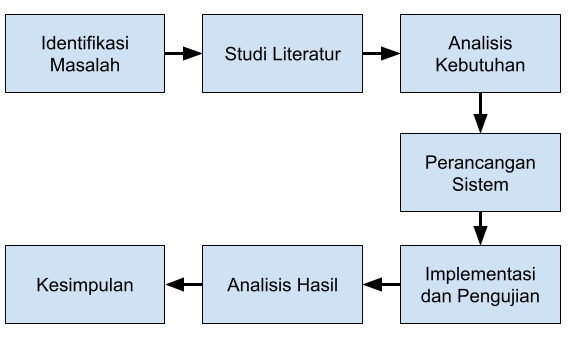
\includegraphics[width=0.8\textwidth]{images/metpen.png}
		\caption{Daigram \textit{experimental design}}
	\end{figure}

\end{adjustwidth}
\begin{adjustwidth}{20pt}{}
	\hspace\parindent
	Berikut merupakan alur tahapan yang dilakukan dalam penelitian ini.
	Pada gambar 3.1, dapat diketahui tahapan penelitian yang akan diterapkan
	pada penelitian ini, yaitu:
\end{adjustwidth}
\begin{adjustwidth}{20pt}{}
	\subsection{Identifikasi Masalah}
	\vspace{-3mm}
	\begin{adjustwidth}{20pt}{}
		Tahapan awal untuk melakukan penelitian merupakan identifikasi masalah. Pada
		tahapan ini, permasalahan yang diidentifikasi mengenai manajemen konfigurasi
		di GNU/Linux untuk mempersingkat waktu konfigurasi dan membuat sistem yang
		terdeklarasi. Peneliti akan membuat konfigurasi sistem operasi GNU/Linux
		menggunakan Ansible dan NixOS dengan kebutuhan yang sama dengan tujuan untuk
		membandingkan efisiensi kecepatan penerapan alat manajemen konfigurasi.
	\end{adjustwidth}
\end{adjustwidth}
\begin{adjustwidth}{20pt}{}
	\subsection{Studi Literatur}
	\vspace{-3mm}
	\begin{adjustwidth}{20pt}{}
		Peneliti mencari literatur yang relevan untuk menjadi referensi pendukung dalam
		penelitian. Literatur yang digunakan dalam penelitian ini berhubungan
		dengan penerapan manajemen konfigurasi yang didapat dari berbagai macam
		sumber seperti buku, artikel, jurnal nasional maupun internasional.
	\end{adjustwidth}
\end{adjustwidth}
\begin{adjustwidth}{20pt}{}
	\subsection{Analisis Kebutuhan}
	\vspace{-3mm}
	\begin{adjustwidth}{20pt}{}
		Tahap ini bertujuan untuk mendapatkan pemahaman yang menyeluruh dan terperinci
		tentang kebutuhan utama sistem seperti yang didefinisikan agar tujuan
		tercapai, yang kemudian secara jelas didefinisikan, ditinjau dan disepakati
		bersama.
	\end{adjustwidth}
\end{adjustwidth}
\begin{adjustwidth}{20pt}{}
	\subsection{Perancangan Sistem}
	\vspace{-3mm}
	\begin{adjustwidth}{20pt}{}
		Perancangan dilakukan dengan menerapkan manajemen konfigurasi pada mesin
		virtual agar mendapatkan hasil waktu yang dibutuhkan untuk menerapkan
		konfigurasi. Berikut flowchart proses dari penerapan konfigurasi yang akan
		dibuat:
		\begin{figure}[!htb]
			\centering
			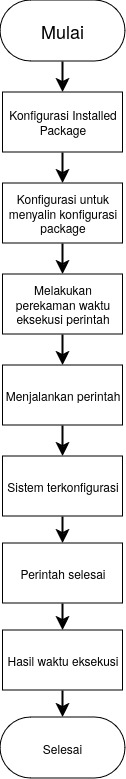
\includegraphics[width=0.2\textwidth]{images/flow.jpg}
			\caption{\textit{flowchart} manajemen konfigurasi}
		\end{figure}
	\end{adjustwidth}
\end{adjustwidth}
\newpage
\begin{adjustwidth}{20pt}{}
	\subsection{Implementasi dan Pengujian}
	\vspace{-3mm}
	\begin{adjustwidth}{20pt}{}
		Pada tahap ini, rancangan konfigurasi yang sudah dibuat akan
		diimplementasikan sesuai alur kerja konfigurasi yang telah dibuat pada
		lingkungan mesin virtual agar lebih efisien dan lebih terisolasi. Instalasi
		dan konfigurasi dilakukan sesuai referensi dokumentasi dari masing-masing
		alat manajemen konfigurasi. Kustomisasi dari perangkat lunak yang
		diperlukan tergantung pada kebutuhan penelitian. Parameter pengujian yang
		akan dilakukan adalah menguji kecepatan waktu eksekusi dan \textit{reproducibility} dari
		masing-masing alat manajemen konfigurasi.
	\end{adjustwidth}
\end{adjustwidth}
\begin{adjustwidth}{20pt}{}
	\subsection{Analisis Hasil}
	\vspace{-3mm}
	\begin{adjustwidth}{20pt}{}
		Pada tahap ini, hasil dari implementasi dan pengujian akan dianalisis untuk
		mengetahui kecepatan penerapan konfigurasi dan konsistensi alat manajemen
		konfigurasi.Untuk mengetahui waktu yang dibutuhkan oleh alat manajemen
		konfigurasi untuk menerapkan konfigurasi, akan digunakan perintah “time”.
		Untuk mengetahui konsistensi penerapan, akan dilihat berdasarkan versi
		paket yang di install dalam rentan waktu yang berbeda.
	\end{adjustwidth}
\end{adjustwidth}

\begin{adjustwidth}{20pt}{}
	\subsection{Kesimpulan}
	\vspace{-3mm}
	\begin{adjustwidth}{20pt}{}
		Tahapan terakhir dalam penelitian ini akan dilakukan penarikan kesimpulan
		dan pemberian saran dari seluruh penelitian yang telah dilakukan
		berdasarkan rumusan masalah yang telah dijelaskan sebelumnya. Hasil dari
		pengujian alat manajemen konfigurasi dapat menjadi jawaban dari masalah
		yang telah dijelaskan, serta data dari penelitian diharapkan berguna dalam
		efisiensi dan konsistensi penerapan manajemen konfigurasi sistem operasi
		GNU/Linux dan dapat menjadi referensi penelitian berikutnya.
	\end{adjustwidth}
\end{adjustwidth}
\vspace{3mm}
\section{Analisis Kebutuhan}
\vspace{-3mm}
\begin{adjustwidth}{20pt}{}
	Analisis kebutuhan merupakan analisis yang dibutuhkan untuk menentukan detail
	kebutuhan pada penelitian analisis perbandingan manajemen konfigurasi sistem
	operasi GNU/Linux antara Ansible dengan NixOS. Penelitian ini mengotomasi
	konfigurasi sistem operasi GNU/Linux dan membuat sistem menjadi terdeklarasi.
	Sehingga dibutuhkan perangkat-perangkat yang dapat mendukung agar penelitian
	ini berjalan sesuai tujuan. Berikut merupakan kebutuhan yang dibagi menjadi
	beberapa bagian, yaitu:
\end{adjustwidth}
\begin{adjustwidth}{20pt}{}
	\subsection{Kebutuhan perangkat keras \{\textit{hardware}\}}
	\vspace{-2mm}
	\begin{adjustwidth}{20pt}{}
		Perangkat keras yang diperlukan guna tujuan penelitian yaitu Laptop sebagai
		uji coba dengan spesifikasi berikut:
	\end{adjustwidth}
	\begin{adjustwidth}{4mm}{}
		\begin{tabular}{ll}
			Processor      & : Intel Core i5 11400H        \\
			RAM            & : 24 GB                       \\
			SSD            & : 1 TB                        \\
			Sistem Operasi & : NixOS 23.11 (Tapir) x86\_64 \\
		\end{tabular}
	\end{adjustwidth}
\end{adjustwidth}
\begin{adjustwidth}{20pt}{}
	\subsection{Kebutuhan perangkat lunak\{\textit{software}\} }
	\vspace{-2mm}
	\begin{adjustwidth}{20pt}{}
		Perangkat lunak berfungsi untuk pengoperasian sistem pada penelitian ini.
		Pada penelitian ini, sistem operasi yang digunakan berbasis GNU/Linux.\\
		\begin{longtable}[r]{|c|p{2cm}|>{\raggedright\arraybackslash}p{4.7cm}|}
			\caption{Kebutuhan perangkat lunak} \tabularnewline  \hline
			\textbf{No.} & \textbf{Nama Perangkat Lunak} & \textbf{Keterangan}                                                       \\
			\endfirsthead
			\textbf{No.} & \textbf{Nama Perangkat Lunak} & \textbf{Keterangan}                                                       \\
			\hline
			\endhead
			\hline
			1            & Ansible                       & Alat yang digunakan untuk manajemen konfigurasi                           \\
			\hline
			2            & NixOS                         & Sistem Operasi dengan fitur manajemen konfigurasi                         \\
			\hline
			3            & Ubuntu Server 24.04 LTS       & Sistem Operasi yang digunakan untuk target Ansible                        \\
			\hline
			4            & Nix Flakes                    & Alat yang digunakan untuk manajemen \textit{inputs} pada NixOS            \\
			\hline
			5            & Home Manager                  & Alat yang digunakan untuk manajemen konfigurasi level pengguna pada NixOS \\
			\hline
			6            & \textit{time}                 & Alat yang digunakan untuk mencatat lama waktu eksekusi perintah           \\
			\hline
		\end{longtable}
	\end{adjustwidth}
\end{adjustwidth}

\section{Perancangan Sistem}
\vspace{-3mm}
\begin{adjustwidth}{20pt}{}
	Perancangan sistem dilakukan untuk membuat desain perencanaan arsitektur
	sistem yang akan dibangun dapat berjalan sesuai dengan tujuan penelitian.
	\subsection{Perancangan Virtual Machine}
	\begin{adjustwidth}{20pt}{}
		Perancangan sistem pada penelitian ini secara keseluruhan menggunakan dua
		\textit{virtual machine}, yang terdiri dari satu \textit{instance} Debian
		12 minimal sebagai host dan target Ansible. \textit{Virtual machine} kedua
		merupakan guest kosong yang akan digunakan sebagai instalasi NixOS minimal.
	\end{adjustwidth}
	\begin{table}[!htbp]
		\caption{Spesifikasi Instance}
		\begin{center}

			\begin{tabular}{|l|l|}
				\hline
				\multicolumn{2}{|c|}{Instance Target Ansible}      \\
				\hline
				Sistem Operasi           & Ubuntu Server 24.04 LTS \\
				\hline
				Processor                & 2                       \\
				\hline
				Memory                   & 4 GB                    \\
				\hline
				Storage                  & 50 GB                   \\
				\hline
				Jumlah \textit{instance} & 3                       \\
				\hline
				\multicolumn{2}{|c|}{Instance Target NixOS}        \\
				\hline
				Sistem Operasi           & NixOS 23.11             \\
				\hline
				Processor                & 2                       \\
				\hline
				Memory                   & 4 GB                    \\
				\hline
				Storage                  & 50 GB                   \\
				\hline
				Jumlah \textit{instance} & 3                       \\
				\hline
			\end{tabular}
		\end{center}
	\end{table}
	\subsection{Perancangan Topologi}
	\begin{adjustwidth}{20pt}{}
		\hspace\parindent
		Perancangan topologi untuk penelitian ini adalah dengan sistem master dan
		target. Sistem ini akan membuat satu perangkat sebagai pusat kendali dari
		beberapa target yang menjadi endpoint dari manajemen konfigurasi.\\
		\begin{figure}[H]
			\centering
			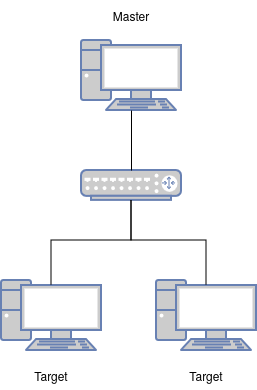
\includegraphics[width=3cm]{images/topologi.png}
			\captionof{figure}{Topologi Pengujian}
		\end{figure}
		Dengan topologi ini, diharapkan penerapan manajemen konfigurasi terpusat
		dan dapat diterapkan di dua mesin target dan memiliki hasil akhir yang sama
		dan konsisten antar mesin.\\
	\end{adjustwidth}
\end{adjustwidth}
\section{Perancangan Pengujian}
\begin{adjustwidth}{20pt}{}
	\hspace\parindent
	Perancangan pengujian pada penelitian ini akan melakukan instalasi berbagai
	macam perangkat lunak. Perangkat lunak yang diinstall adalah tmux, vim,
	neovim, htop. Kemudian akan dilakukan beberapa konfigurasi perangkat lunak
	yaitu konfigurasi untuk tmux, vim, neovim, openssh, firewall.

	Kemudian akan dihadirkan service tambahan yaitu berupa \textit{web server}
	menggunakan Nginx. Nginx juga akan dikonfigurasi untuk menampilkan
	\textit{website} sederhana yang kode sumbernya diambil dari
	\textit{repository} Github.
	\begin{figure}[H]
		\centering
		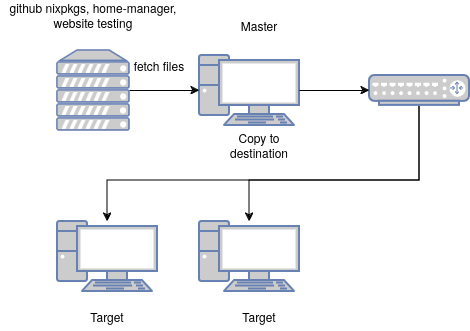
\includegraphics[width=\textwidth]{images/Topologi-NixOS.png}
		\caption{Alur Penerapan Konfigurasi NixOS}
	\end{figure}

	Pada gambar 3.3 merupakan alur penerapan konfigurasi menggunakan NixOS.
	Master akan melakukan \textit{clone} dari \textit{repository} nixpkgs,
	home-manager dan website-testing untuk mengambil konfigurasi sistem serta
	file \textit{website} yang akan di \textit{deploy}. Kemudian \textit{master}
	akan melakukan build untuk konfigurasi keseluruhan sistem sehingga
	menghasilkan nix derivation yang membentuk NixOS. Hasil dari derivation
	tersebut kemudian akan di \textit{copy} dan diterapkan ke dua mesin target.

	\begin{figure}[H]
		\centering
		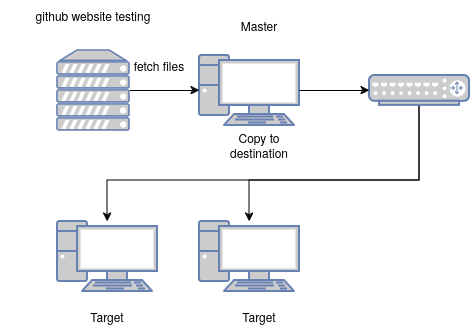
\includegraphics[width=\textwidth]{images/Topologi-Ansible.png}
		\caption{Alur Penerapan Konfigurasi Ansible}
	\end{figure}
	Pada gambar 3.5 merupakan alur penerapan konfigurasi menggunakan Ansible.
	\textit{Master} akan melakukan \textit{clone} dari \textit{repository} github
	website-testing. Kemudian \textit{master} akan mulai menerapkan konfigurasi
	untuk target dan menginstall semua paket yang di definisikan dan melakukan
	konfigurasi yang diinginkan. Setelah konfigurasi sistem selesai diterapkan
	kemudian Ansible akan menyalin file \textit{website} yang ada di master ke
	target.

	Setiap kali perintah untuk melakukan konfigurasi di eksekusi, waktu eksekusi
	akan dicatat menggunakan perintah “time”. Eksekusi akan dilakukan secara
	berulang untuk mendapatkan rata-rata waktu yang dibutuhkan untuk menerapkan
	konfigurasi.\\
\end{adjustwidth}
\section{Time Schedule}
\begin{adjustwidth}{20pt}{}
	Berikut \textit{time schedule} yang penulis susun sebagai acuan pelaksanaan
	kegiatan:
	\begin{table}[H]
		\caption{Time Schedule}
		\begin{tabular}{|p{2cm}|c|c|c|c|c|c|}
			\hline
			\multicolumn{1}{|c|}{\multirow{2}{*}{\centering{\textbf{Kegiatan}}}} & \textbf{2023}     & \multicolumn{5}{|c|}{\textbf{2024}}                                                                                 \\
			\cline{2-7}
			                                                                     & Des               & Jan                                 & Feb               & Mar               & Apr               & Mei               \\
			\hline
			Identifikasi Masalah                                                 & \cellcolor{green} &                                     &                   &                   &                   &                   \\
			\hline
			Studi Literatur                                                      &                   & \cellcolor{green}                   &                   &                   &                   &                   \\
			\hline
			Analisis Kebutuhan                                                   &                   & \cellcolor{green}                   &                   &                   &                   &                   \\
			\hline
			Perancangan Sistem                                                   &                   &                                     & \cellcolor{green} & \cellcolor{green} &                   &                   \\
			\hline
			Implementasi dan Pengujian                                           &                   &                                     &                   &                   & \cellcolor{green} &                   \\
			\hline
			Analisis Hasil                                                       &                   &                                     &                   &                   &                   & \cellcolor{green} \\
			\hline
			Kesimpulan                                                           &                   &                                     &                   &                   &                   & \cellcolor{green} \\
			\hline
		\end{tabular}
	\end{table}

\end{adjustwidth}
\chapter{HASIL PENELITIAN DAN PEMBAHASAN}
Hasil dari penelitian peneliti berupa data-data terkait waktu eksekusi yang
dibutuhkan untuk penerapan manajemen konfigurasi dari eksekusi nixos-rebuild
dan ansible-playbook. Peneliti membangun dua jenis konfigurasi, yaitu
konfigurasi untuk NixOS dan Ansible. Untuk konfigurasi NixOS menggunakan flake
untuk mencapai \textit{reproducibility} dan Home-Manager untuk mengkonfigurasi
aplikasi pengguna.

Untuk konfigurasi Ansible dibuat semirip mungkin dengan konfigurasi NixOS.
Perbedaan nya adalah metode file konfigurasi pada Ansible menggunakan
ansible.posix.synchronize dan ansible.builtin.copy untuk menyalin /
mensinkronisasi file konfigurasi setiap aplikasi dan \textit{services}.
\vspace{3mm}
\section{Implementasi}
\begin{adjustwidth}{20pt}{}
	\subsection{Struktur Konfigurasi NixOS}
	\begin{adjustwidth}{20pt}{}
		\vspace{-3mm}
		Untuk struktur konfigurasi yang digunakan adalah sebagai berikut:
		\begin{figure}[H]
			\centering
			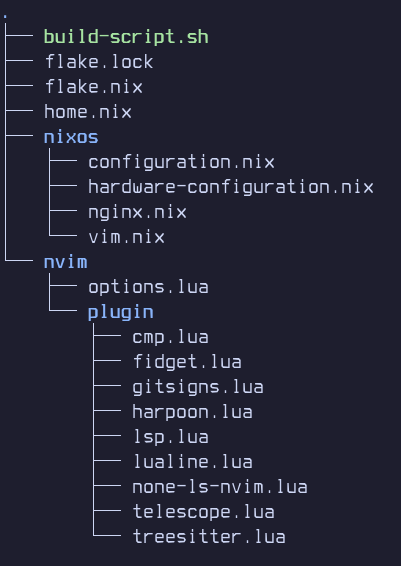
\includegraphics[width=0.4\textwidth]{images/directory-tree.png}
			\caption{Directory-tree}
		\end{figure}

		Dalam konfigurasi ini, flake.nix dan flake.lock diletakkan di parent
		directory yang memang menjadi basis untuk dieksekusinya perintah
		"nixos-rebuild switch -{}- flake .\#nixos-vm", dimana opsi -{}-flake sendiri
		terdiri dari flake-uri[\#hostname]

		\begin{code}
			\begin{minted}{nix}
        {
          inputs = {
            nixpkgs.url = "github:nixos/nixpkgs/nixos-23.11";
            home-manager = {
              url = "github:nix-community /home-manager/release-23.11";
              inputs.nixpkgs.follows = "nixpkgs";
            };
            testing-website = {
              url = "github:rizqirazkafi/testing-website";
              flake = false;
            };
          };
        }
      \end{minted}
			\caption{flake inputs}
		\end{code}


		Flake.nix berisi tiga inputs yang dimana terdiri dari nixpkgs, home-manager,
		dan testing-website. Hasil dari inputs tadi digunakan dalam output untuk
		sistem yang didefinisikan dalam nixosConfiguration dengan nixos-vm sebagai
		hostname dari sistem.

		\begin{code}[H]
			\begin{minted}{nix}
        {
          outputs = { self, nixpkgs, home-manager, ... }@inputs:
          let
          system = "x86_64-linux";
          pkgs = import nixpkgs {
            inherit system;
            config = { allowUnfree = true; };
          };
          in
          {
            nixosConfigurations = {
              nixos-vm = nixpkgs.lib.nixosSystem {
                specialArgs = { inherit inputs system pkgs; };
                modules = [ ./nixos/configuration.nix ];
              };
            };
          };
        }
      \end{minted}
			\caption{flake outputs}
		\end{code}

		Dengan flake, versi paket yang dihasilkan dalam output tidak akan berubah
		baik dari channel maupun hash. Ini dikarenakan, informasi tersebut disimpan
		dalam flake.lock. Dengan ini, sistem yang dihasilkan akan konsisten dan
		dapat disebut sebagai sistem yang \textit{reproducible}.

		Contoh konten flake.lock adalah sebagai berikut:

		\begin{code}
			\begin{minted}{json}
        {
          "nodes": {
            "nixpkgs": {
              "locked": {
                "lastModified": 1708702655,
                "narHash": "sha256-qxT5jSxxx",
                "owner": "nixos",
                "repo": "nixpkgs",
                "rev": "c5101e457206dd437330d283d6626944e28794b3",
                "type": "github"
              },
              "original": {
                "owner": "nixos",
                "ref": "nixos-23.11",
                "repo": "nixpkgs",
                "type": "github"
              },
            },
          }
        }
      \end{minted}
			\caption{nixpkgs lock di flake.lock}
		\end{code}


	\end{adjustwidth}
	\subsection{Konfigurasi inti configuration.nix}
	\vspace{-3mm}
	\begin{adjustwidth}{20pt}{}
		File configuration.nix berisikan konfigurasi sistem seperti \textit{system
			packages, services, user packages, ssh option, }dan lain-lain. File ini
		bisa dibilang merupakan file inti dari konfigurasi sistem secara menyeluruh
		dimana file inilah yang di evaluasi oleh nixos-rebuild. Semua module yang
		dibutuhkan sistem harus di referensikan dalam file ini agar konfigurasi
		dapat diterapkan ke sistem.
		Ini merupakan sebagian konten file configuration.nix yang digunakan pada
		penelitian ini:

		\begin{code}
			\begin{minted}{nix}
        {inputs, pkgs, ... }: {
          nixpkgs.config.allowUnfree = true;
          environment.systemPackages = with pkgs; [
            lazygit
            tmux
            vim
            neovim
            wget
            git
            home-manager
            htop
            ranger
            ripgrep
            ansible
          ];
          security.pam.enableSSHAgentAuth = true;
          security.pam.enableSSHAgentAuth = true;
          services.openssh = {
            enable = true;
            ports = [ 9005 ];
            settings.PasswordAuthentication = false;
          };
        }
      \end{minted}
		\end{code}
	\end{adjustwidth}
	\subsection{Home Manager}
	\vspace{-3mm}
	\begin{adjustwidth}{20pt}{}
		Untuk konfigurasi Home Manager, ada beberapa yang dimasukkan yaitu :
		\begin{enumerate}
			\item LSP server yang dibutuhkan untuk Neovim
			\item plugin untuk Neovim
			\item userName dan userEmail git
			\item enableCompletion untuk BASH
		\end{enumerate}

		Berikut merupakan sebagian dari konfigurasi yang dipakai untuk penelitian ini:

		\begin{code}
			\begin{minted}{nix}
        {config, pkgs, inputs, ...}:
        {
          home.username = "rizqirazkafi";
          home.homeDirectory = "/home/rizqirazkafi";
          programs.neovim = let
          toLua = str: ''
          lua << EOF
          ${str}
          EOF
          '';
          toLuaFile = file: ''
          lua << EOF
          ${builtins.readFile file}
          EOF
          '';
          in {
            enable = true;
            extraPackages = with pkgs; [
              # list of lsp
              xclip
              luajitPackages.lua-lsp
              rnix-lsp
              ansible-language-server
              nodePackages.bash-language-server
              shfmt
              ansible-lint
            ];
            plugins = with pkgs.vimPlugins; [
              vim-tmux-navigator
              nvim-lspconfig
              auto-pairs
              undotree
              {
                plugin = comment-nvim;
                config = toLua ''require("Comment").setup()'';
              }
            ];
          };
        }
      \end{minted}
			\caption{Konfigurasi home.nix untuk Home-Manager}
		\end{code}
	\end{adjustwidth}
	\subsection{Konfigurasi Ansible}
	\vspace{-3mm}
	\begin{adjustwidth}{20pt}{}
		\hspace\parindent
		Untuk Ansible menggunakan konfigurasi yang lebih sederhana dengan menyalin
		file konfigurasi dari vim, neovim, tmux, ssh, dan nginx ke
		\textit{directory} konfigurasi sesuai Filesystem Hierarchial Standard
		(FHS). Untuk paket yang dibutuhkan di definisikan secara \textit{global
			packages} dimana paket di install untuk semua \textit{user}.

		Untuk \textit{Language Server Protocol} (LSP) \textit{server} akan
		ditangani oleh Lazy.nvim dan Mason agar terinstall secara otomatis
		saat Neovim dijalankan.

		Rincian konfigurasinya adalah sebagai berikut:

		\begin{code}
			\begin{minted}{yaml}
        - hosts: all
          become: yes
          become_user: root
          tasks:
          - name: install packages
            package:
              name:
                - hello
                - neovim
                - tmux
                - vim
                - wget
                - ....
      \end{minted}
			\caption{Konfigurasi instalasi paket di Ansible}
		\end{code}

		\begin{code}
			\begin{minted}{yaml}
        - name: copy nginx default config
          ansible.builtin.copy:
            src: default
            dest: /etc/nginx/sites-enabled/default
        - name: copy php8.3-fpm config
          ansible.builtin.copy:
            src: php-demo.conf
            dest: /etc/php/8.3/fpm/pool.d
      \end{minted}
			\caption{Salin konfigurasi paket dan services ke target}
		\end{code}

		\begin{code}
			\begin{minted}{yaml}
        - name: enable nginx
        ansible.builtin.service:
          name: nginx
          state: restarted
      \end{minted}
			\caption{Restart service menggunakan Ansible}
		\end{code}

		Maka dengan kedua alat Manajemen Konfigurasi inilah telah tercapai sistem
		GNU/Linux yang terdeklarasi dimana sistem terdeklarasikan dalam bentuk
		file-file konfigurasi.
	\end{adjustwidth}
\end{adjustwidth}
\newpage
\section{Pengujian}
\begin{adjustwidth}{20pt}{}
	\hspace\parindent
	Tahap pengujian yang dilakukan dalam penelitian ini dimaksudkan untuk mengetahui
	waktu eksekusi yang dibutuhkan dari Ansible dan NixOS untuk menerapkan manajemen
	konfigurasi yang telah dibuat. Pengujian dilakukan dengan menggunakan perintah
	"\textit{time}" pada eksekusi setiap kali dijalankan perintah untuk penerapan manajemen
	konfigurasi.
	\subsection{Pasca Install}
	\begin{adjustwidth}{20pt}{}
		Pengujian dilakukan dengan menjalankan Ansible Playbook dan nixos-rebuild
		ke dua Virtual Machine yang baru saja di install. Tidak ada konfigurasi
		tambahan selain konfigurasi untuk IP menggunakan NetworkManager dan SSH.
		Masing-masing sistem juga berjalan di mode shell tanpa GUI. Pengujian ini
		akan dijalankan sebanyak satu kali.
	\end{adjustwidth}

	\subsubsection{NixOS tanpa cache}
	\begin{adjustwidth}{20pt}{}
		Pada percobaan ini, nixos-rebuild akan mengunduh semua \textit{binary} dan
		\textit{dependency} kemudian akan melakukan \textit{build} berdasarkan
		\textit{derivation} yang telah di definisikan oleh nixpkgs. Hasil dari
		\textit{derivation} berupa \textit{closure} yang disalin ke target.
	\end{adjustwidth}
	\vspace{-3mm}
	\begin{table}[H]
		\begin{center}
			\begin{tabular}[c]{|c|c|c|}
				\hline
				\multicolumn{1}{|c|}{\textbf{real}} &
				\multicolumn{1}{c|}{\textbf{user}}  &
				\multicolumn{1}{c|}{\textbf{sys}}                         \\
				\hline
				2m7.863s                            & 0m8.449s & 0m3.204s \\
				\hline
			\end{tabular}
		\end{center}
		\caption{nixos-rebuild first target}
	\end{table}
	\vspace{-3mm}
	\begin{table}[H]
		\begin{center}
			\begin{tabular}[c]{|c|c|c|}
				\hline
				\multicolumn{1}{|c|}{\textbf{real}} &
				\multicolumn{1}{c|}{\textbf{user}}  &
				\multicolumn{1}{c|}{\textbf{sys}}                           \\
				\hline
				3m23.585s                           & 0m11.772s & 0m11.070s \\
				\hline
			\end{tabular}
		\end{center}
		\caption{nixos-rebuild second target}
	\end{table}
	\subsubsection{NixOS dengan Cache}
	\begin{adjustwidth}{20pt}{}
		Pada percobaan ini, nixos-rebuild akan mengunduh semua \textit{binary} dan
		\textit{dependency} kemudian akan melakukan \textit{build} berdasarkan
		\textit{derivation} yang telah di definisikan oleh nixpkgs. Hasil dari
		\textit{derivation} berupa \textit{closure} yang disalin ke target.
		\vspace{-3mm}
		\begin{table}[H]
			\begin{center}
				\begin{tabular}[c]{|c|c|c|}
					\hline
					\multicolumn{1}{|c|}{\textbf{real}} &
					\multicolumn{1}{c|}{\textbf{user}}  &
					\multicolumn{1}{c|}{\textbf{sys}}                         \\
					\hline
					1m4.684s                            & 0m4.152s & 0m5.701s \\
					\hline
				\end{tabular}
			\end{center}
			\caption{nixos-rebuild first target}
		\end{table}
		\vspace{-3mm}
		\begin{table}[H]
			\begin{center}
				\begin{tabular}[c]{|c|c|c|}
					\hline
					\multicolumn{1}{|c|}{\textbf{real}} &
					\multicolumn{1}{c|}{\textbf{user}}  &
					\multicolumn{1}{c|}{\textbf{sys}}                        \\
					\hline
					1m11.445s                           & 0m4.325s & 0m6.508 \\
					\hline
				\end{tabular}
			\end{center}
			\caption{nixos-rebuild second target}
		\end{table}
	\end{adjustwidth}
	\subsubsection{Ansible Single Target}
	\begin{adjustwidth}{20pt}{}
		Pada percobaan ini, dijalankan menggunakan perintah ansible-playbook dengan
		satu target pada satu waktu. Total target yang di tuju adalah dua.
		\begin{table}[H]
			\begin{center}
				\begin{tabular}[c]{|c|c|c|}
					\hline
					\multicolumn{1}{|c|}{\textbf{real}} &
					\multicolumn{1}{c|}{\textbf{user}}  &
					\multicolumn{1}{c|}{\textbf{sys}}                         \\
					\hline
					3m9.988s                            & 0m8.048s & 0m2.277s \\
					\hline
				\end{tabular}
			\end{center}
			\caption{ansible first target}
		\end{table}
	\end{adjustwidth}
	\subsection{Penerapan ulang setelah pasca install.}
	\begin{adjustwidth}{20pt}{}
		Pengujian ini dilakukan dengan cara menjalankan Ansible Playbook dan nixos-rebuild
		setelah pengujian Pasca Install tanpa perubahan apapun pada file konfigurasi. Pengujian ini
		akan dijalankan sebanyak tiga kali.
	\end{adjustwidth}
	\vspace{-3mm}
	\begin{table}[H]
		\begin{center}
			\begin{tabular}[c]{|c|c|c|}
				\hline
				\multicolumn{1}{|c|}{\textbf{real}} &
				\multicolumn{1}{c|}{\textbf{user}}  &
				\multicolumn{1}{c|}{\textbf{sys}}                         \\
				\hline
				0m4.256s                            & 0m0.192s & 0m0.084s \\
				\hline
				0m2.562s                            & 0m0.192s & 0m0.089s \\
				\hline
				0m2.506s                            & 0m0.200s & 0m0.078s \\
				\hline
			\end{tabular}
		\end{center}
		\caption{nixos-rebuild first target}
	\end{table}
	\begin{table}[H]
		\begin{center}
			\begin{tabular}[c]{|c|c|c|}
				\hline
				\multicolumn{1}{|c|}{\textbf{real}} &
				\multicolumn{1}{c|}{\textbf{user}}  &
				\multicolumn{1}{c|}{\textbf{sys}}                         \\
				\hline
				0m3.868s                            & 0m0.194s & 0m0.087s \\
				\hline
				0m2.670s                            & 0m0.194s & 0m0.087s \\
				\hline
				0m2.658s                            & 0m0.192s & 0m0.008s \\
				\hline
			\end{tabular}
		\end{center}
		\caption{nixos-rebuild second target}
	\end{table}
	\subsection{Penambahan Paket}
	\begin{adjustwidth}{20pt}{}
		Pengujian dilakukan dengan menambahkan paket tambahan yaitu Go compiler.
		Pengujian ini akan dilakukan tiga kali dengan satu kali perubahan pada file
		konfigurasi.
	\end{adjustwidth}
	\vspace{-3mm}
	\begin{table}[H]
		\begin{center}
			\begin{tabular}[c]{|c|c|c|}
				\hline
				\multicolumn{1}{|c|}{\textbf{real}} &
				\multicolumn{1}{c|}{\textbf{user}}  &
				\multicolumn{1}{c|}{\textbf{sys}}                         \\
				\hline
				0m52.362s                           & 0m7.317s & 0m2.315s \\
				\hline
				0m2.674s                            & 0m0.180s & 0m0.092s \\
				\hline
				0m2.550s                            & 0m0.189s & 0m0.090s \\
				\hline
			\end{tabular}
		\end{center}
		\caption{nixos-rebuild first target}
	\end{table}
	\begin{table}[H]
		\begin{center}
			\begin{tabular}[c]{|c|c|c|}
				\hline
				\multicolumn{1}{|c|}{\textbf{real}} &
				\multicolumn{1}{c|}{\textbf{user}}  &
				\multicolumn{1}{c|}{\textbf{sys}}                         \\
				\hline
				0m5.292s                            & 0m0.530s & 0m0.366s \\
				0m2.655s                            & 0m0.202s & 0m0.081s \\
				0m2.635s                            & 0m0.203s & 0m0.072s \\
				\hline
			\end{tabular}
		\end{center}
		\caption{nixos-rebuild second target}
	\end{table}
	\subsection{Penghapusan Paket}
	\begin{adjustwidth}{20pt}{}
		Pengujian dilakukan dengan menghapus paket yaitu Go compiler.
		Pengujian ini akan dilakukan tiga kali dengan satu kali perubahan pada file
		konfigurasi.
	\end{adjustwidth}
	\begin{table}[H]
		\begin{center}
			\begin{tabular}[c]{|c|c|c|}
				\hline
				\multicolumn{1}{|c|}{\textbf{real}} &
				\multicolumn{1}{c|}{\textbf{user}}  &
				\multicolumn{1}{c|}{\textbf{sys}}                         \\
				\hline
				0m2.685s                            & 0m0.200s & 0m0.081s \\
				\hline
				0m2.540s                            & 0m0.198s & 0m0.081s \\
				\hline
				0m2.569s                            & 0m0.192s & 0m0.084s \\
				\hline
			\end{tabular}
		\end{center}
		\caption{nixos-rebuild first target}
	\end{table}
	\begin{table}[H]
		\begin{center}
			\begin{tabular}[c]{|c|c|c|}
				\hline
				\multicolumn{1}{|c|}{\textbf{real}} &
				\multicolumn{1}{c|}{\textbf{user}}  &
				\multicolumn{1}{c|}{\textbf{sys}}                         \\
				\hline
				0m2.785s                            & 0m0.225s & 0m0.080s \\
				\hline
				0m2.768s                            & 0m0.217s & 0m0.081s \\
				\hline
				0m2.781s                            & 0m0.234s & 0m0.069s \\
				\hline
			\end{tabular}
		\end{center}
		\caption{nixos-rebuild second target}
	\end{table}
\end{adjustwidth}

\addcontentsline{toc}{chapter}{\textbf{DAFTAR PUSTAKA}}
\printbibliography[title={DAFTAR PUSTAKA}]
\end{document}
